\documentclass{beamer}
\usetheme{boxes}
\usecolortheme{rose}
\usefonttheme{default}
\usepackage[german]{babel}

\title{\textbf{\huge{Biometric Crypto-Systems}} \\[1ex]}
\author{Felix Baumann, Ravinder Sangar, Jonas Winkler}
%\date{\footnotesize{xx.06.2020}}

\begin{document}
\begin{frame}
	\titlepage
\end{frame}

\begin{frame}{Inhalt}
	\tableofcontents
\end{frame}

\section{Einleitung}
\subsection{Was sind Biometrische Kryptosysteme}
\begin{frame}{Biometrische Kryptosysteme}
	\begin{itemize}
		\item Biometrische Daten sind biologische Messwerte, die Personen eindeutig identifizieren\\ [2ex]
		\item Bsp: Fingerabdruckscan, Gesichtserkennung, Irisscan \\ [2ex]
		\item Biometrische Kryptosysteme verbinden Kryptographie mit Biometrie \\ [2ex]
	\end{itemize}
	\hspace{19mm}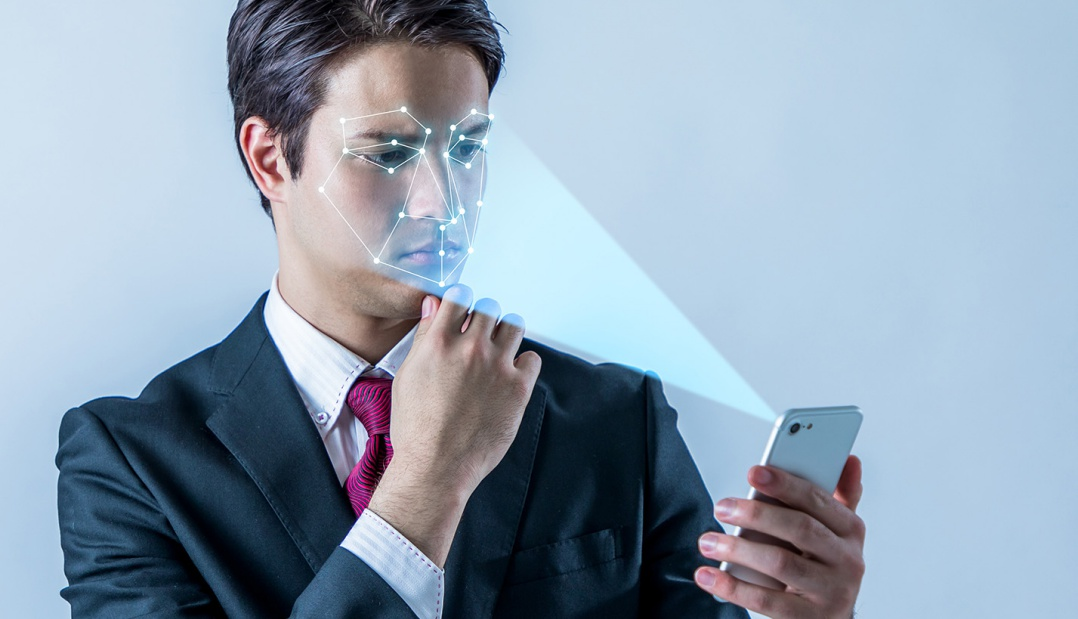
\includegraphics [height = 4 cm ]{gesichtserkennung.jpg} \\
	\hspace{18mm}\tiny{Quelle: \textit{\tiny{https://www.cancom.info/2019/03/gesichtserkennung-technologie/}}}
\end{frame}

\begin{frame}{Funktionsweise}
	\hspace{17mm}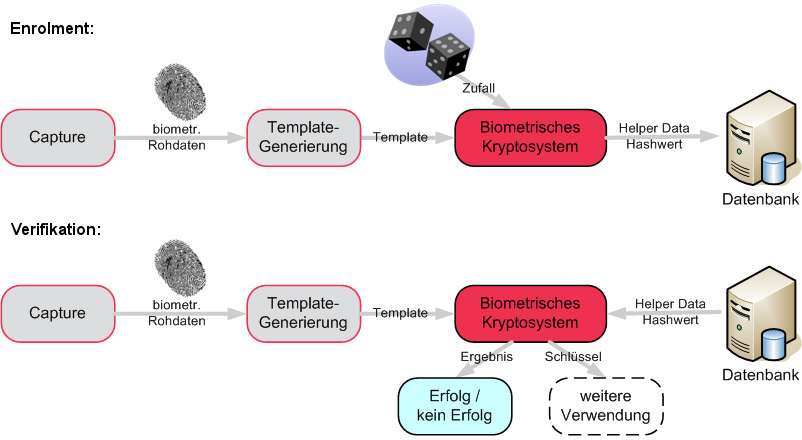
\includegraphics [height = 4 cm ]{08-6-052-1.jpg} \\
	\hspace{20mm}\tiny{Quelle: \textit{\tiny{http://2014.kes.info/archiv/online/images/08-6-052-1-400.jpg}}}
\end{frame}

\begin{frame}{Inhalt}
	\tableofcontents
\end{frame}

\section{Ursprung}
\subsection{Idee hinter Biometrie}
\begin{frame}{Idee hinter Biometrie}
	\begin{itemize}
		\item Erste Biometrie war der Fingerabdruck
		\item Vor 4000 Jahren wurde mit Fingerabdrücken unterzeichnet
		\item Henry Fauld fand heraus, dass Fingerabdrücke individuell sind \\[2ex]
	\end{itemize}
	\hspace{38mm}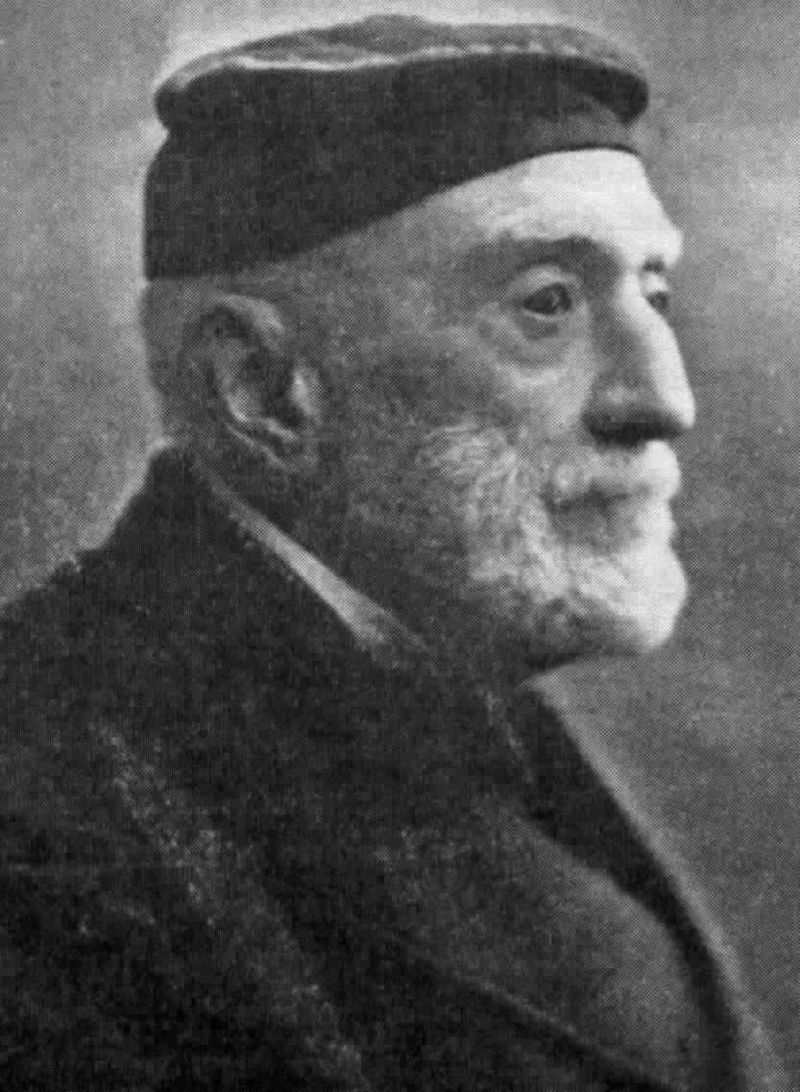
\includegraphics [height = 4 cm ]{Henry_Faulds.jpg} \\
	\hspace{40mm} \tiny{Quelle: \textit{\tiny{de.wikipedia.org}}}
\end{frame}

\subsection{Heutige Verwendung}
\begin{frame}{Heutige Verwendung}
	\begin{itemize}
		\item Fingerabdrücke werden heute in Forensik eingesetzt
		\item Gesichtserkennung bei einigen Smartphone und in Flughäfen
		\item Schlüssel für Gebäude werden von Fingerabdruckscane abgelöst
		\item Biometrischer Pass wird weltweit eingesetzt: Bild des Gesichts und 2 Fingerabdruckbilder \\[2ex]
	\end{itemize}
	\hspace{39mm}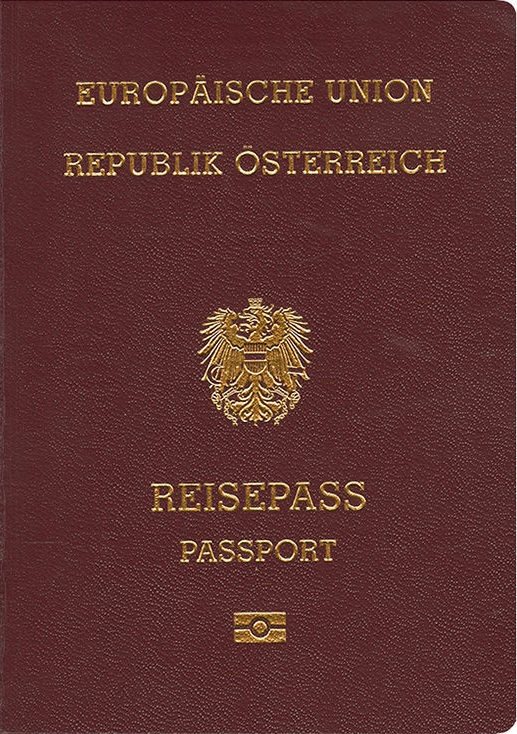
\includegraphics [height = 4 cm ]{Reisepass_at.jpg} \\
	\hspace{41mm} \tiny{Quelle: \textit{\tiny{wikimedia.org}}}

\end{frame}

\section{Problematik}
\subsection{Gefahr vor Hackangriffen}
\subsection{Biometrische Daten sind unveränderbar}
\subsection{Duplikation von biometrischen Daten}
\begin{frame}{Problematik}
	\begin{itemize}
		\item Alle biometrischen Daten, die gesammelt wurden, können gehackt werden
		\item Biometrische Daten können nicht verändert werden, wie ein Passwort
		\item Duplikation von Daten: Fingerabdrücke können im Alltag unbemerkt abgenommen werden, Hochauflösende Fotos von Gesichtern
	\end{itemize}
\end{frame}

\section{Biometric Template Protection}
\begin{frame}{Biometric Template Protection}
	\begin{itemize}
		\item Fingerabdruck nicht \"anderbar $\rightarrow$ muss gesch\"utzt werden
		\item Template nicht direkt gespeichert
		\item umgewandelt in „Protected Templates“
		\item reicht aus f\"ur Authentifizierung
	\end{itemize}
\end{frame}
\section{Fuzzy Commitment}
\subsection{Funktionsweise}
\begin{frame}{Fuzzy Commitment}
	\begin{itemize}
		\item Commitment-Schema generell
		\begin{itemize}
			\item $G : C\times X \rightarrow W$
			\item \textit{binding}-Eigenschaft
			\item \textit{hiding}-Eigenschaft
		\end{itemize}
		\item Fuzzy Commitment besteht aus 2 Phasen:
		\begin{itemize}
			\item \textit{Enrollment}-Phase: Initialisierung und Anlegen des Templates \& Schl\"ussels
			\item \textit{Authentication}-Phase: Verfahren zur Authentifizierung 
		\end{itemize}
	\end{itemize}
\end{frame}
\begin{frame}{Enrollment I}
	\begin{itemize}
		\item zuf\"alliger Wert f\"ur Schl\"ussel $s$, One-Way-Hashfunktion $h(s)$ generiert
		\item Schl\"ussel $s$ in Hamming-Code $c$ umgeschrieben
	\end{itemize}
	\hspace{10mm}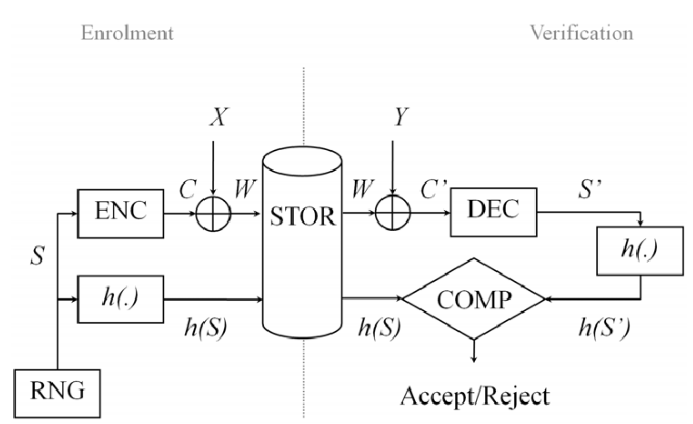
\includegraphics[height=5cm]{fcs.png}\\
	\tiny{Quelle: \textit{\tiny{$https://www.cosy.sbg.ac.at/~uhl/biometrics_slides.pdf$}}}
\end{frame}
\begin{frame}{Hamming-Code I}
	\begin{itemize}
		\item an jede $2^{x}$-te Position kommt Parit\"atsbit
		\item alle \textbf{Stellen} mit Wert 1 werden verxort
		\item Ergebnis stellt Wert für Parit\"atsbits dar
	\end{itemize}
	\vspace{10mm}
\includegraphics[height=1.5cm]{hamming_zug.png}\\
	\tiny{Quelle: \textit{\tiny{$https://www.cybersicherheit.guru/der-hamming-code/$}}}
\end{frame}
\begin{frame}{Hamming-Code II - Beispiel}
	\begin{itemize}
		\item zu codieren: 1101
		\item f\"uge Parit\"atsbit an Positionen 1, 2 und 4 ein $\rightarrow$ 110\textcolor{red}{x}1\textcolor{red}{xx}
		\item Stellen, an denen Wert 1 ist miteinander verXORen $\rightarrow$ Stellen 7, 6, 3
		\item 7 	== \textcolor{blue}{1}1\textcolor{green}{1}
		\item 6 == \textcolor{blue}{1}1\textcolor{green}{0}
		\item 3 == \textcolor{blue}{0}1\textcolor{green}{1}
		\item xor == \textcolor{blue}{0}1\textcolor{green}{0} $\rightarrow$ Parit\"atsbits haben Werte \textcolor{red}{1}, \textcolor{red}{0}, \textcolor{red}{0}
		\item Codewort: 110\textcolor{red}{1}1\textcolor{red}{00}
	\end{itemize}
\end{frame}
\begin{frame}{Enrollment II}
	\begin{itemize}
		\item Template (als Bitstring) $x$ XOR $c$ ergibt „Safe“ $w$
	\end{itemize}
	\hspace{10mm}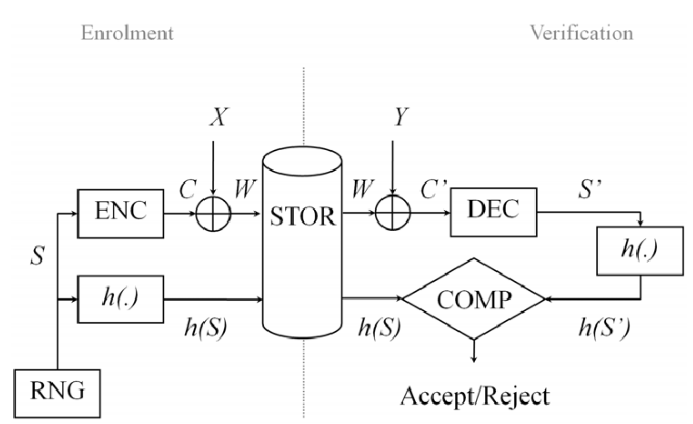
\includegraphics[height=5cm]{fcs.png}\\
	\tiny{Quelle: \textit{\tiny{$https://www.cosy.sbg.ac.at/~uhl/biometrics_slides.pdf$}}}
\end{frame}
\begin{frame}{Authentication I}
	\begin{itemize}
		\item neues Template $y$ wird eingelesen (User hält Finger an Sensor)
		\item $w \oplus y = c'$ (Kandidaten-Codewort)
	\end{itemize}
	\hspace{10mm}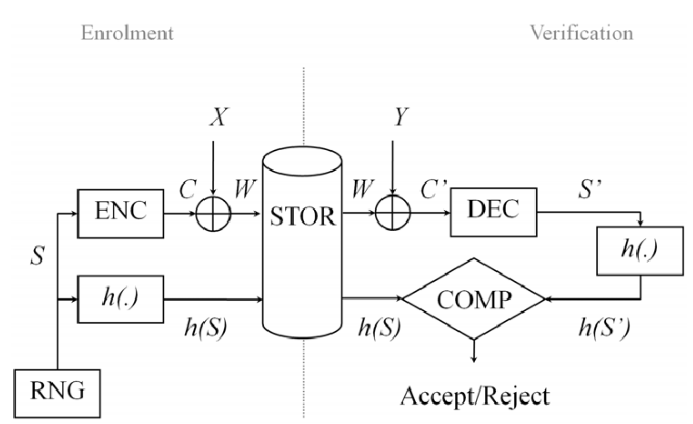
\includegraphics[height=5cm]{fcs.png}\\
	\tiny{Quelle: \textit{\tiny{$https://www.cosy.sbg.ac.at/~uhl/biometrics_slides.pdf$}}}
\end{frame}
\begin{frame}{Hamming-(De)code}
	\begin{itemize}
		\item $c'$ muss nun decodiert werden $\rightarrow$ es werden erneut die Stellen aller 1en verXORt
		\item Beispiel: $c'$ = 00\textcolor{red}{1}00\textcolor{red}{1}0
		\item 2 == 010
		\item 5 == 101
		\item xor == 111 $\rightarrow$ bedeutet an der Stelle 3 ist ein Bitfehler aufgetreten, er kann korrigiert werden
		\item wenn Ergebnis == 0 $\rightarrow$ fehlerfreie Übertragung
		\item nur 1-Bit-Fehler kann korrigiert werden
	\end{itemize}
\end{frame}
\begin{frame}{Authentication II}
	\begin{itemize}
		\item Parit\"atsbits werden wieder entfernt $\rightarrow$ Kandidatenschl\"ussel $s'$
		\item Einsetzen von $s'$ in $h(.)$, wenn $h(s) == h(s')$ $\rightarrow$ Authentifizierung erfolgreich
	\end{itemize}
	\hspace{10mm}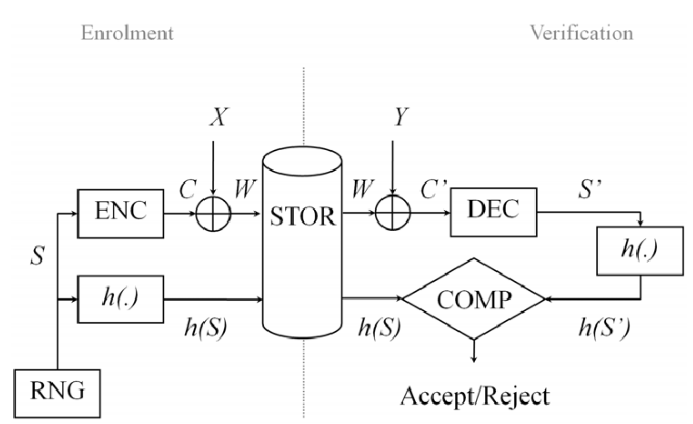
\includegraphics[height=5cm]{fcs.png}\\
	\tiny{Quelle: \textit{\tiny{$https://www.cosy.sbg.ac.at/~uhl/biometrics_slides.pdf$}}}
\end{frame}
\subsection{Vor- und Nachteile}
\begin{frame}{Fuzzy Commitment}
	\begin{itemize}
		\item Vorteile	\\[1ex]
		\begin{itemize}
			\item entstehende Unsch\"arfe kann ausgeglichen werden
			\item Template selbst wird nicht gespeichert $\rightarrow$ gut gesch\"utzt
		\end{itemize}
		\item Nachteile \\[1ex]
		\begin{itemize}
			\item Template muss als Bitstring dargestellt werden (möglichst kurz, da nur 1-Bit-Fehler erkannt werden)
			\item L\"ange des Template-Bitstrings $x$ muss mit jener des Keys $s$ übereinstimmen, wegen XOR
		\end{itemize}
	\end{itemize}
\end{frame}


\section{Fuzzy Vault}
\subsection{Funktionsweise}
\begin{frame}{Fuzzy Vault}
	\begin{itemize}
		\item Fingerabdrücke sind nicht zu 100\% reproduzierbar\\[1.5 ex]
		\item Konzept das Fehler tolleriert?\\[1.5 ex]
	\end{itemize}
\end{frame}
\begin{frame}{Fuzzy Vault}
	\begin{itemize}
		\item Alice möchte wissen ob jemand ihre Interessen teilt \\[1.5 ex]
		\item Alice sichert Interessen in einem Save\\[1.5 ex]
		\item Bob hat ähnliche Interessen\\[1.5 ex]
		\item Bob kann den Save entsperren\\[1.5 ex]
	\end{itemize}
\end{frame}

\begin{frame}{Prinzip}
		\hspace{10mm}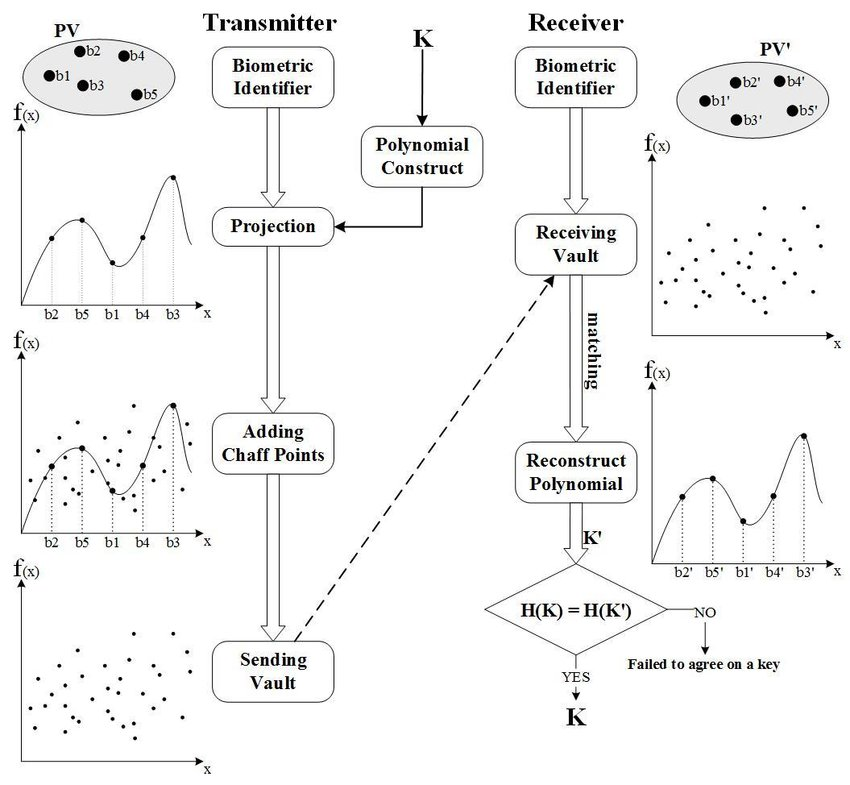
\includegraphics [height = 8cm ]{fuzzy_vault.png} \\
		\tiny{Quelle: \textit{\tiny{$https://www.researchgate.net/figure/Key-distribution-solution-based-on-fuzzy-vault-		scheme-112_fig1_321080531/$}}}
\end{frame}

\begin{frame}{Biometric Template}
		\hspace{10mm}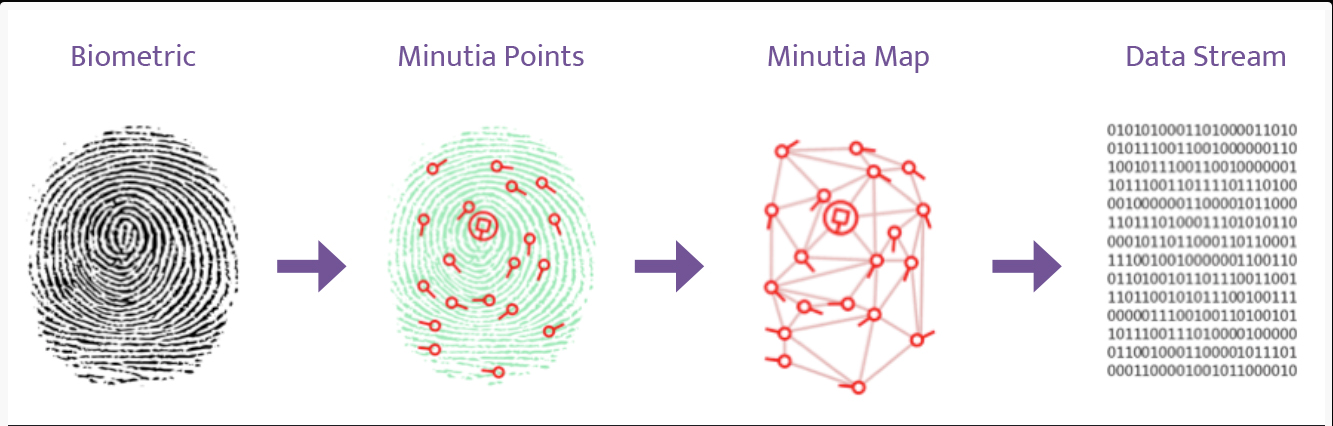
\includegraphics [height =3.5cm ]{template.PNG} \\
		\tiny{Quelle: \textit{\tiny{$http://www.tellen.co.nz/biometric-doorkeeper/prettyPhoto[gallery6320]/0$}}}
\end{frame}
\begin{frame}{Parameter}
	\begin{itemize}
		\item Universum $F$\\[1.5 ex]
		\item Secret $s$\\[1.5 ex]
		\item Polynomfunktion p \\[1.5 ex]
		\item Bob kann den Save entsperren
	\end{itemize}
\end{frame}
\subsubsection{LOCK}
\begin{frame}{LOCK}
		\hspace*{10mm}$ X,R\rightarrow \emptyset$ \newline
		\hspace*{10mm}$s \rightarrow p$\newline
		\hspace*{10mm}$for \; i=1 \; to \; t $\newline
		\hspace*{15mm}$(a_{i}, p(a_{i})) \rightarrow (x_{i}, y_{i})$\newline
		\hspace*{15mm}$X\bigcup \{x_{i}\} \rightarrow X$\newline
		\hspace*{15mm}$R\bigcup \{(x_{i},y_{i})\} \rightarrow R$\newline
		\hspace*{10mm}$for \; i=t+1 \; to \; r$\newline
		\hspace*{15mm}$x_{i} \in F - X$\newline
		\hspace*{15mm}$y_{i} \in F - \{ (x_{i},y_{i} \}$\newline
		\hspace*{15mm}$R\cup \{(x_{i},y_{i})\} \rightarrow R$\newline
		\hspace*{10mm}$return\;R$\newline
\end{frame}
\begin{frame}{Prinzip}
		\hspace{10mm}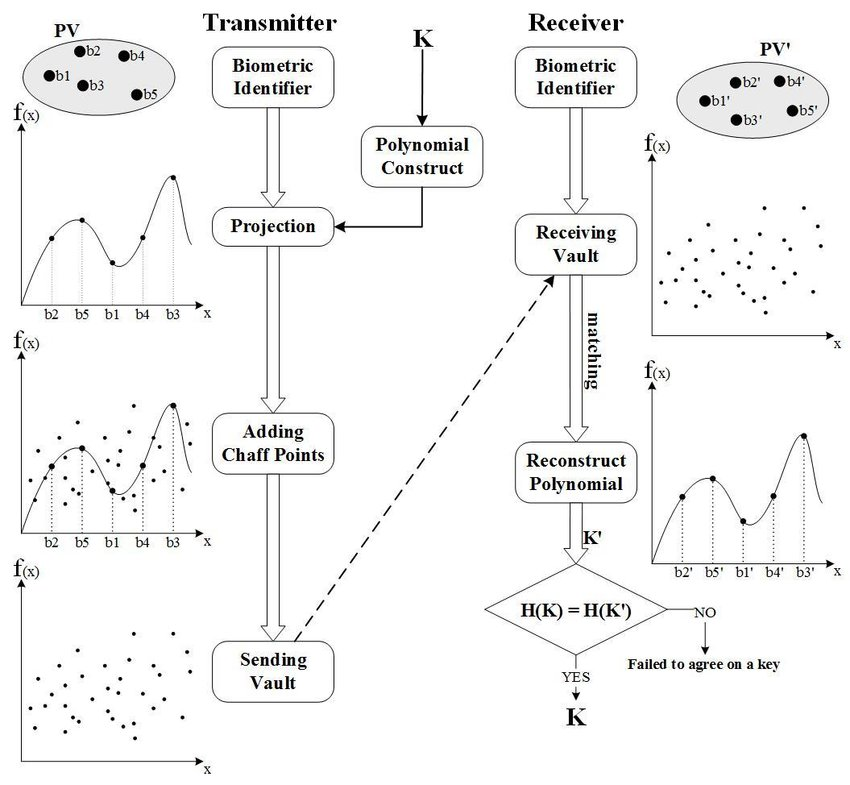
\includegraphics [height = 8cm ]{fuzzy_vault.png} \\
		\tiny{Quelle: \textit{\tiny{$https://www.researchgate.net/figure/Key-distribution-solution-based-on-fuzzy-vault-		scheme-112_fig1_321080531/$}}}
\end{frame}
\subsubsection{UNLOCK}
\begin{frame}{UNLOCK}
	\hspace*{10mm}$ Q \rightarrow \emptyset$ \\[1ex]
	\hspace*{10mm}$for \; i=1 \; to \; t $\\[1ex]
	\hspace*{15mm}$R \xrightarrow{\text{ $b_{i}, \circ $}} (x_{i}, y_{i})$\\[1ex]
	\hspace*{15mm}$Q\bigcup (x_{i},y_{i}) \rightarrow Q$\\[1ex]
	\hspace*{10mm}$RS_{DECODE}(k,Q) \rightarrow s'$\\[1ex]
	\hspace*{10mm}$return\; s' $\\[1ex]
\end{frame}
\subsection{Vor- und Nachteile}
\begin{frame}{Vor- und Nachteile}
\begin{itemize}
		\item Vorteile	\\[1ex]
		\begin{itemize}
			\item Fehler der Sensoren/Finger werden toleriert
			\item Chaff-Points bestimmen die Sicherheit \\[3ex]
		\end{itemize}
		\item Nachteile \\[1ex]
		\begin{itemize}
			\item eventuell weniger Sicherheit gegenüber anderen Verschlüsselungssysteme bei wenigen Chaff-Points
			\item Risiko für hohe Komplexität
		\end{itemize}
	\end{itemize}
\end{frame}
\begin{frame}
\huge{Vielen Dank für Ihre Aufmerksamkeit}
\end{frame}
\end{document}
